\section{Schreibweisen}

\subsection{Fischer Projektion}
\label{sec:fischer}
\begin{itemize}
    \item längste C-Kette von oben nach unten
    \item höchst oxidiertes C-Atom nach oben
\end{itemize}

Dabei ist zu beachten, dass durch die Fischerprojektion Enantiomere und Diastomere erfasst werden können. 
Wenn bei dem folgenden Stoff die OH-Gruppe auf der linken Seite wäre, wäre dies ein Diastomer zu dem Stoff. 
Wären alle asymmetrischen C-Atome gespiegelt wäre es ein Enantiomer. \\
D-Glucose:

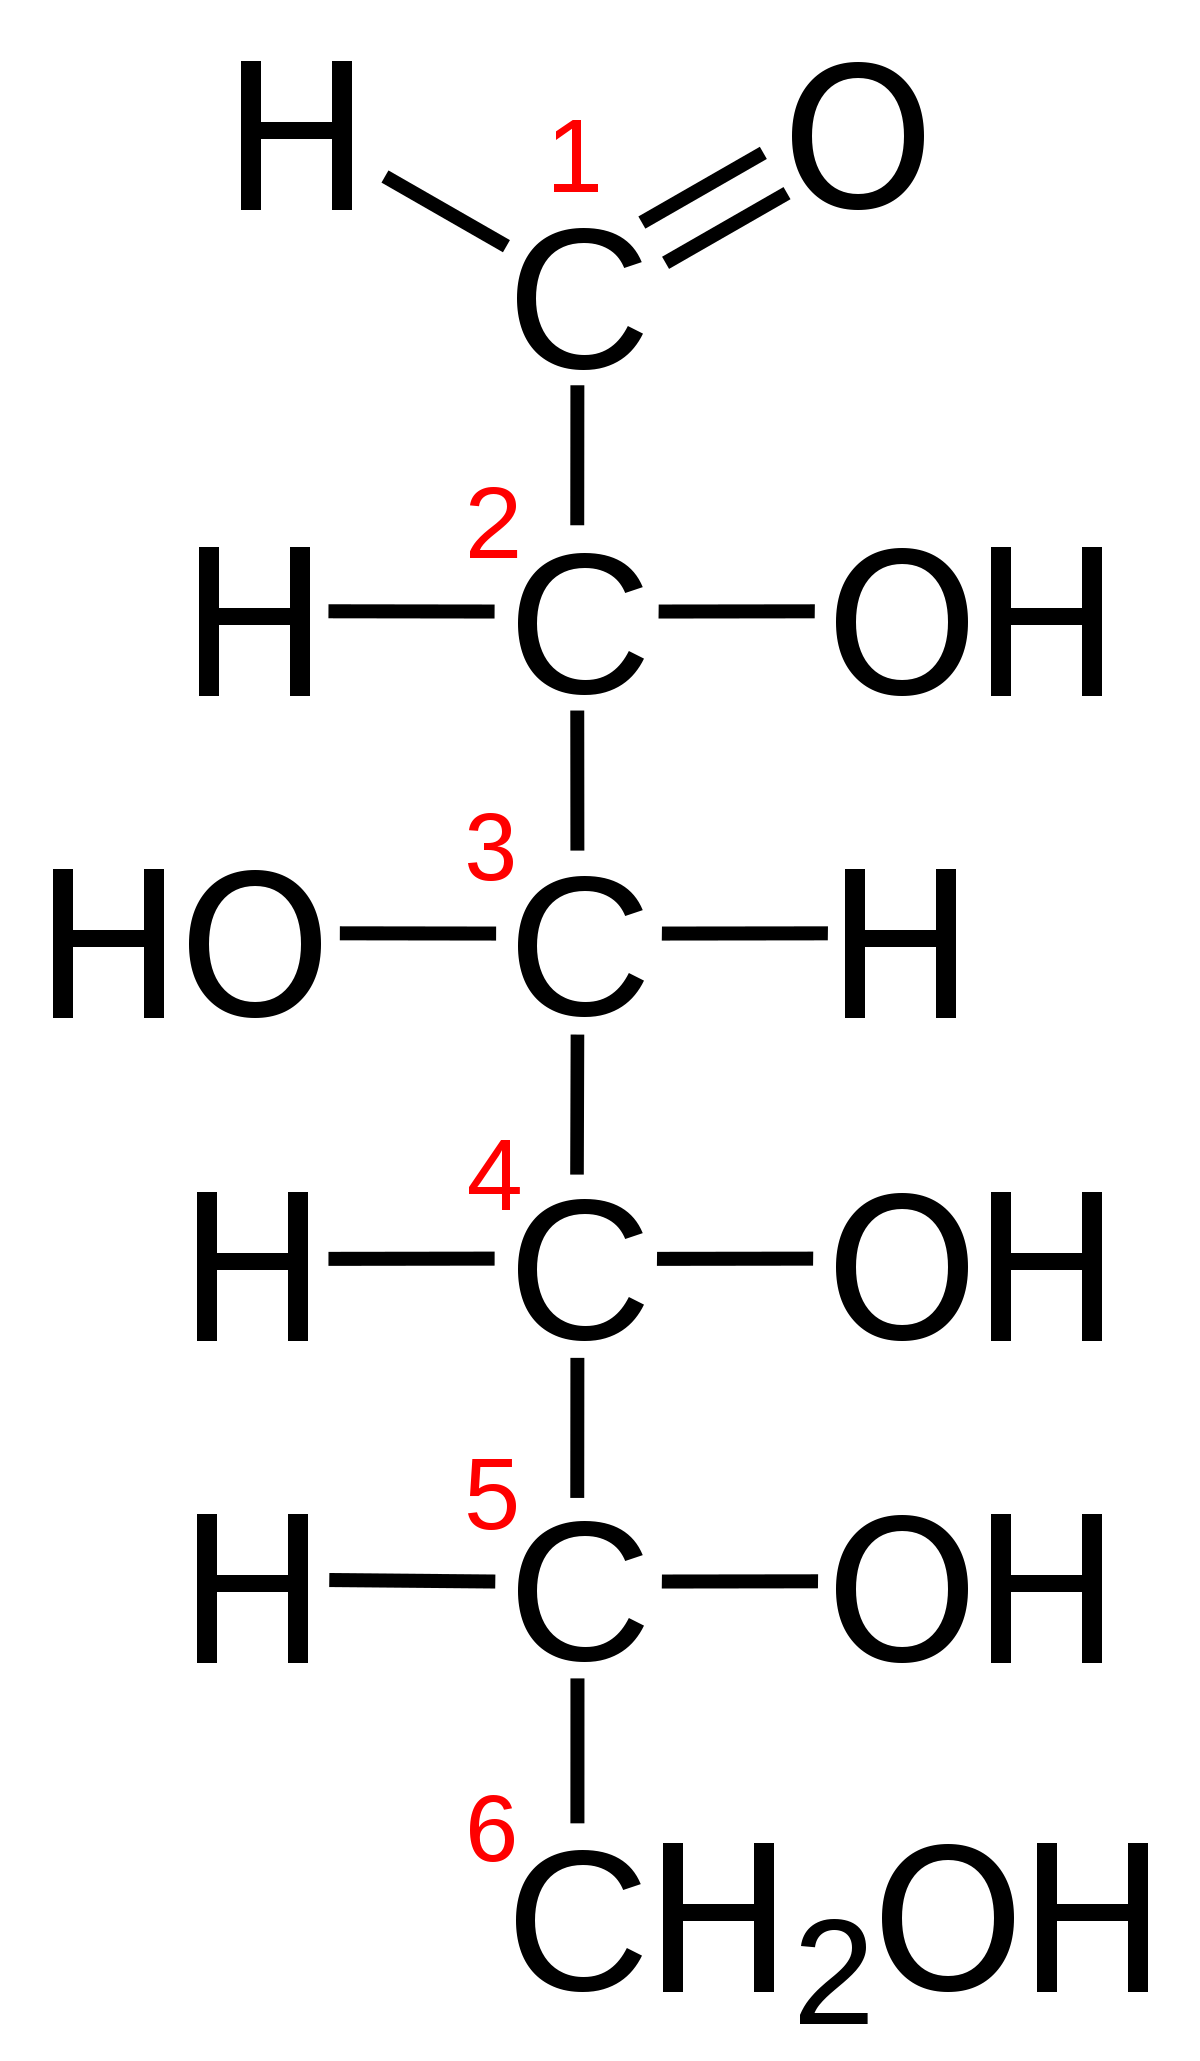
\includegraphics[scale=0.06]{media/naturstoffe/fischer.png}

\subsection{Haworth Projektion}
\label{sec:haworth}
D-Glucose:

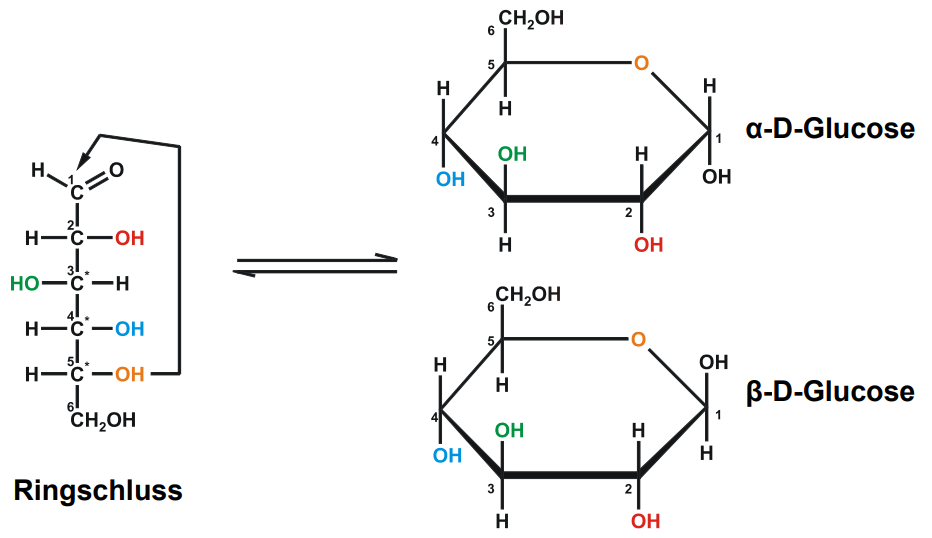
\includegraphics[scale=0.86]{media/naturstoffe/haworth.png}

